\documentclass[xetex,mathserif,serif]{beamer}
\usepackage{polyglossia}
\setdefaultlanguage[babelshorthands=true]{russian}
\usepackage{minted}
\usepackage{tabu}

\useoutertheme{infolines}

\usepackage{fontspec}
\setmainfont{FreeSans}
\newfontfamily{\russianfonttt}{FreeSans}

\usepackage{forest}
\usetikzlibrary{arrows}

\setbeamertemplate{blocks}[rounded][shadow=false]
\setbeamercolor*{block title example}{fg=green!50!black,bg=green!20}
\setbeamercolor*{block body example}{fg=black,bg=green!10}

\setbeamercolor*{block title alerted}{fg=red!50!black,bg=red!20}
\setbeamercolor*{block body alerted}{fg=black,bg=red!10}

\tabulinesep=0.7mm

\title{Стайлгайд, процесс компиляции}
\author[Юрий Литвинов]{Юрий Литвинов \newline \textcolor{gray}{\small\texttt{yurii.litvinov@gmail.com}}}

\date{14.09.2018}

\begin{document}
	
	\frame{\titlepage}
	
	\begin{frame}
		\frametitle{Стайлгайд}
		\begin{itemize}
			\item Программы пишутся для людей, а не для компьютера
			\item “Школьник-стайл” именования переменных (a, b, c1)
			\item Отступы!
			\item Пробелы!
			\item Правила именования
			\begin{itemize}
				\item Переменные со строчной, типы с заглавной
			\end{itemize}
			\item Компилироваться без предупреждений
			\item Не должно быть копипаста
			\item \url{http://se.math.spbu.ru/SE/Members/ylitvinov/styleguide}
		\end{itemize}
	\end{frame}

	\begin{frame}
		\frametitle{Процесс компиляции С++}
		\begin{center}
			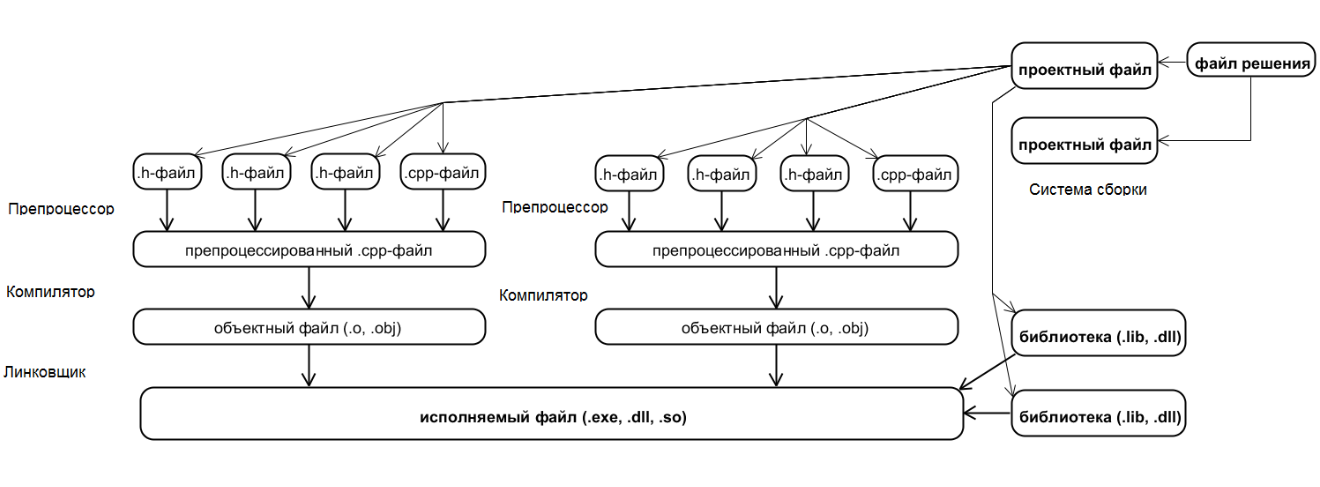
\includegraphics[width=0.8\textwidth]{compilation.png}
		\end{center}
	\end{frame}

\end{document}

